%%% License: Creative Commons Attribution Share Alike 4.0 (see https://creativecommons.org/licenses/by-sa/4.0/)


%%%%%%%%%%%%%%%%%%%%%%%%%%%%%%%%%%%%%%%%%

%----------------------------------------------------------------------------------------
%	PACKAGES AND OTHER DOCUMENT CONFIGURATIONS
%----------------------------------------------------------------------------------------

\documentclass[a4paper]{article}

\usepackage{amssymb}
\usepackage{enumerate}
\usepackage[usenames,dvipsnames]{color}
\usepackage{fancyhdr} % Required for custom headers
\usepackage{lastpage} % Required to determine the last page for the footer
\usepackage{extramarks} % Required for headers and footers
\usepackage[usenames,dvipsnames]{color} % Required for custom colors
\usepackage{graphicx} % Required to insert images
\usepackage{listings} % Required for insertion of code
\usepackage{courier} % Required for the courier font
\usepackage[table]{xcolor}
\usepackage{amsfonts,amsmath,amsthm,parskip,setspace,url}
\usepackage[section]{placeins}
\usepackage[a4paper]{geometry}
\usepackage[USenglish]{babel}
\usepackage[utf8]{inputenc}
\usepackage{tikz}


% Margins
\topmargin=-0.45in
\evensidemargin=0in
\oddsidemargin=0in
\textwidth=6.5in
\textheight=9.0in
\headsep=0.6in

\linespread{1.1} % Line spacing



%----------------------------------------------------------------------------------------
%   FORMATTING
%----------------------------------------------------------------------------------------
% Set up the header and footer
\pagestyle{fancy}
\lhead[c]{\textbf{{\color[rgb]{.5,0,0} K{\o}benhavns\\Universitet }}} % Top left header
\chead{\textbf{{\color[rgb]{.5,0,0} \Class }}\\ \hmwkTitle  } % Top center head
\rhead{\instructor \\ \theprofessor} % Top right header
\lfoot{\lastxmark} % Bottom left footer
\cfoot{} % Bottom center footer
\rfoot{Page\ \thepage\ of\ \protect\pageref{LastPage}} % Bottom right footer
\renewcommand\headrulewidth{0.4pt} % Size of the header rule
\renewcommand\footrulewidth{0.4pt} % Size of the footer rule


% Other formatting stuff
%\setlength\parindent{12pt}
\setlength{\parskip}{5 pt}
%\theoremstyle{definition} \newtheorem{ex}{\textbf{\Large{Exercise & #}\\}}
\usepackage{titlesec}
\titleformat{\section}[hang]{\normalfont\bfseries\Large}{Problem \thesection:}{0.5em}{}




%----------------------------------------------------------------------------------------
%	NAME AND CLASS SECTION
%----------------------------------------------------------------------------------------
\newcommand{\hmwkTitle}{Exercises for Lecture 5} % Assignment title
\newcommand{\Class}{Mechanism Design} % Course/class
\newcommand{\instructor}{Fall 2024} % TA
\newcommand{\theprofessor}{Prof. Egor Starkov} % Professor




%----------------------------------------------------------------------------------------
%   SOLUTIONS
%----------------------------------------------------------------------------------------
\newif\ifsolutions
\solutionstrue




\begin{document}

\begin{center}
		\LARGE\textbf{Exercises for Lecture 5:\\ gVCG, AGV.}
\end{center}



\section{Efficient public good provision 3}

Consider the usual public project problem setup:
There is a society of $N$ people. They must collectively decide whether to implement a public project. Let $k \in \{0,1\}$ denote the outcome of this decision: $k=1$ if project is implemented, $k=0$ otherwise. Every person $i$ has some private valuation $\theta_i \in \mathbb{R}$ for the project, positive or negative. Preferences are linear, so $i$'s utility can be written as
$$
u_i(x,\theta) = \theta_i k(\theta) - t_i(\theta).
$$
Here $x=(k,t)$ stands for some direct mechanism which prescribes outcome $k(\theta) \in \{0,1\}$ and payment profile $t(\theta)$ given profile of reports $\theta$.

Assume now that players' valuations are independently distributed according to $\theta_i \sim U[-\hat{\theta},\hat{\theta}]$ for all $i$, and that the public project has some known social cost $c > 0$. 
All players' outside options are zero: $\underline{U}_i(\theta_i)=0$.

Derive the gVCG transfers.

\ifsolutions
\section*{Solution}
LCT for any $i$ is $\tilde{\theta}_i = -\hat{\theta}$ (you do not actually need to calculate the expectation to find it, since the expression that $\tilde{\theta}_i$ minimizes is weakly monotone in $\theta_i$ -- i.e., one of the edges of the support is the solution). The gVCG transfers are then given by
\begin{align*}
	t_i^{gVCG}(\theta) &= \max \left\{0, \sum_{j\neq i}\theta_j -\hat{\theta} - c \right\} - \left(\sum_{j\neq i}\theta_j -c\right) \cdot \mathbb{I} \left\{ \sum_{j=1}^N \theta_j - c > 0 \right\}
	\\
	&= \begin{cases}
		0	&	\text{ if } \sum_{j=1}^N \theta_j - c \leq 0,
		\\
		-\left(\sum_{j\neq i}\theta_j - c \right)	&	\text{ if }	\sum_{j\neq i} \theta_j - \hat{\theta} - c \leq 0 < \sum_{j=1}^N \theta_j - c,
		\\
		-\hat{\theta}	&	\text{ if } \sum_{j\neq i}\theta_j -\hat{\theta} - c > 0.
	\end{cases}
\end{align*}
\fi



\section{AGV and public goods}

Consider the public good provision problem (again). Suppose now that there are only two individuals: $i=1,2$, their valuations for the public project are $\theta_i \sim i.i.d. U[-1,1]$, and the cost is $c \in [0,1]$ (known to all agents).

\begin{enumerate}
	\item Calculate the AGV transfers for this problem.
	\item Do the players' payments to the mechanism cover the project cost $c$ if and only if the project is implemented? (I.e., is the mechanism exactly budget balanced once we account for the project costs?)
\end{enumerate}

\ifsolutions
\section*{Solution}
Note: the lectures are somewhat vague, so you can get somewhat different expressions in part 1 depending on how exactly you approach the problem. The answer to part 2 should, however, be qualitatively the same in all of those cases.

The $\tilde{t}$ are as follows: for $i=1,2$,
\begin{align*}
	\tilde{t}_i(\theta_i) &= \mathbb{E}_{\theta_j} \left[ (\theta_j - c) \cdot \mathbb{I} \{ \theta_1+\theta_2 \geq c \} \right]
	\\
	&= \int_{\min\{c-\theta_i, 1\}}^{1} (\theta_j -c) \frac{1}{2} d\theta_j 
	\\
	&= \frac{1}{4} \left[ (c-1)^2 - \theta_i^2 \right] \cdot \mathbb{I} \{ \theta_i \geq c-1 \};
\end{align*}
and the actual transfers are then $t_i^{AGV}(\theta) = \tilde{t}_j(\theta_j) - \tilde{t}_i(\theta_i)$ for $i=1,2$, which evaluates to 
\begin{align*}
	t_i^{AGV}(\theta) = \begin{cases}
		\frac{\theta_i^2 - \theta_j^2}{4} & \text{ if } \theta_i,\theta_j \geq c-1 \text{ (region I)},
		\\
		\frac{(c-1)^2 - \theta_j^2}{4} & \text{ if } \theta_j \geq c-1 > \theta_i \text{ (region II)},
		\\
		\frac{\theta_i^2 - (c-1)^2}{4} & \text{ if } \theta_i \geq c-1 > \theta_j \text{ (region III)},
		\\
		0 & \text{ if } c-1 > \theta_i,\theta_j \text{ (region IV)}.
	\end{cases}
\end{align*}
\begin{figure}
	\begin{center} 
		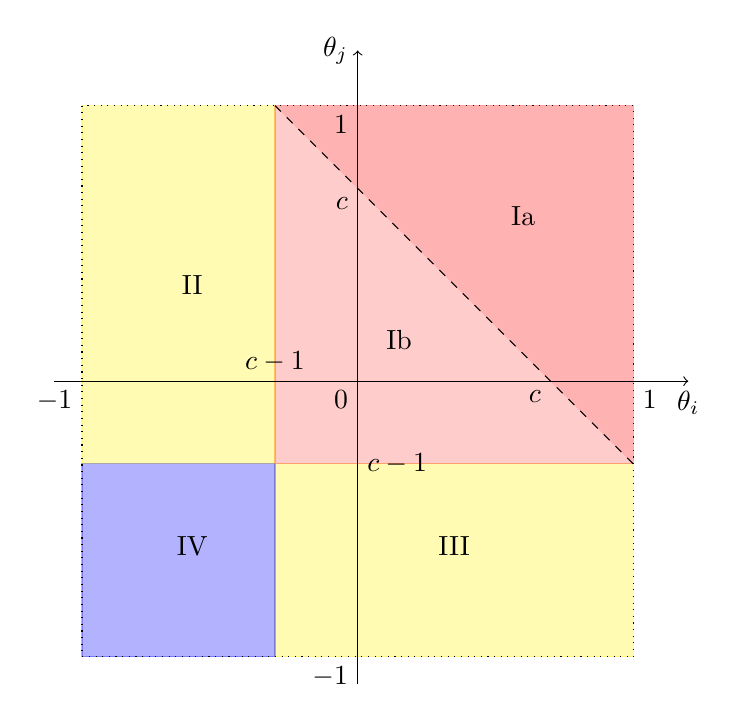
\begin{tikzpicture}[scale=3.5]
			%regions
			\filldraw[yellow, opacity=0.3] (-0.3,-0.3) -| (-1,1) -| (-0.3,-0.3);
			\filldraw[yellow, opacity=0.3] (-0.3,-0.3) -| (1,-1) -| (-0.3,-0.3);
			\filldraw[red, opacity=0.3] (-0.3,1) -| (1,1) -| (1,-0.3);
			\filldraw[red, opacity=0.2] (-0.3,1) -| (-0.3,-0.3) -| (1,-0.3);
			\filldraw[blue, opacity=0.3] (-0.3,-0.3) -| (-1,-1) -| (-0.3,-0.3);
			\draw (0.6,0.6) node{Ia};
			\draw (0.15,0.15) node{Ib};
			\draw (-0.6,0.35) node{II};
			\draw (0.35,-0.6) node{III};
			\draw (-0.6,-0.6) node{IV};
			
			% axes 
			\draw[->] (-1.1,0) -- (1.2,0) node[below]{$\theta_i$};
			\draw[->] (0,-1.1) -- (0,1.2) node[left]{$\theta_j$};
			\draw (0,0) node[below left]{$0$};
			\draw (0,1) node[below left]{$1$};
			\draw (0,-1) node[below left]{$-1$};
			\draw (1,0) node[below right]{$1$};
			\draw (-1,0) node[below left]{$-1$};
			
			\draw (-0.3,0) node[above ]{$c-1$};
			\draw (0,-0.3) node[right ]{$c-1$};
			\draw (0.7,0) node[below left]{$c$};
			\draw (0,0.7) node[below left]{$c$};
			
			% bounding box
			\draw[dotted] (1,-1) |- (-1,1) |- (1,-1);
			
			% lines
			\draw[dashed] (-0.3,1) -- (1,-0.3);
		\end{tikzpicture}
		\caption{regions for AGV transfers}
		\label{fig:AGV}
	\end{center}
\end{figure}

The regions are plotted in Figure \ref{fig:AGV}. Note that the public project is implemented only in region Ia, but the two agents' transfers sum up to zero there, same as in all other regions. Therefore, the AGV mechanism does not cover the project cost.
At this point you might think that this is because you need to compute $\tilde{t}_0$ and somehow include it in the players' payments. However, regardless of how you split this $\tilde{t}_0$ across agents, payments in regions Ia and Ib will always be continuous at the border (since $\tilde{t}_0$ would just add some constant to agents' payments), whereas to cover the cost of the project exactly, the sum of payments must be larger by $c$ in Ia than in Ib.
%\begin{align*}
%\tilde{t}_0 &= \mathbb{E}_{\theta_1,\theta_2} \left[ (\theta_1+\theta_2) \mathbb{I} \{ \theta_1+\theta_2 \geq c \} \right]
%\\
%&= \int_{c-1}^1 \left[ \int_{c-\theta_i}^1 (\theta_1+\theta_2) d\theta_2 \right] d\theta_1 
%\\
%&= \frac{4+c^3}{3}.
%\end{align*}
\fi 



\section{Myerson-Satterthwaite theorem}

Consider the \textbf{bilateral trade} problem discussed in class: one buyer, one seller, one item. The seller's valuation for the item is given by his private type $\theta_S \sim U[0,1]$, and the buyer's valuation is given by his private type $\theta_B \sim U[0,1]$, independent of $\theta_S$. The outside options are given by $\underline{U}_S({\theta}_S)={\theta}_S$ and $\underline{U}_B({\theta}_B)=0$ respectively. The utilities of the two players are Euclidean and are given by:
\begin{align*}
	u_S &= v(k,\theta_S)-t_S(\theta)=\theta_S (1-k)-t_S(\theta)
	\\
	u_B &= v(k,\theta_B)-t_B(\theta)=\theta_B k-t_B(\theta)
\end{align*}
where $k(\theta) \in [0,1]$ is the probability of trade given type profile $\theta$. The designer would like to create an efficient market for these players (i.e., implement the efficient allocation rule)

Derive the gVCG transfers for this problem. Show that the resulting mechanism is not ex ante budget balanced (not even weakly).


\ifsolutions
\section*{Solution}
It is straightforward to see that the efficient allocation rule $k^*$ is given by:
\begin{align*}
	k^*= \begin{cases}
		1 & \text{ if } \theta_S \leq \theta_B \\ 
		0 & \text{ if } \theta_S > \theta_B
	\end{cases}
\end{align*}
Our next step is to construct the gVCG transfers that implement the efficient allocation. They are given by:
\begin{align*}
	t_S^{gVCG} = v_B(k^*(\tilde{\theta}_S,\theta_B),\theta_B) + v_S(k^*(\tilde{\theta}_S,\theta_B),\tilde{\theta}_S) - \\
	-v_B(k^*(\theta_S,\theta_B),\theta_B) - \underline{U}_S(\tilde{\theta}_S)
	\\
	t_B^{gVCG} = v_S(k^*(\tilde{\theta}_B,\theta_S),\theta_S) + v_B(k^*(\tilde{\theta}_B,\theta_S),\tilde{\theta}_B) - \\
	-v_S(k^*(\theta_B,\theta_S),\theta_S) - \underline{U}_B(\tilde{\theta}_B)
\end{align*}
Noticing that $v_B(k^*(\theta))+v_S(k^*(\theta)) = \max \{\theta_B,\theta_S\}$ and plugging in the efficient allocation $k^*$ and the outside options $\underline{U}_i$, we get
\begin{align*}
	t_S^{gVCG} &= \max\{\tilde{\theta}_S,\theta_B\} - \theta_B k^*(\theta_S,\theta_B) - \tilde{\theta}_S
	\\
	t_B^{gVCG} &= \max\{\tilde{\theta}_B,\theta_S\} - \theta_S \left(1 - k^*(\theta_S,\theta_B)\right)
\end{align*}

The least charitable types $\tilde{\theta}_i$ of each player are defined as:
\begin{align*}
	\tilde{\theta}_i &\in \arg \min_{\theta_i \in \Theta_i} \left\{ \mathbb{E}_{\theta_{-i}} \left[ v_B (k^*(\theta_i,\theta_{-i}),\theta_j) + v_S (k^*(\theta_i,\theta_{-i}),\theta_j) - \underline{U}_i (\theta_i) \right] \right\}
	\\
	\Rightarrow \tilde{\theta}_B &\in \arg \min_{\theta_B \in [0,1]} \left\{ \mathbb{E}_{\theta_S} \left[ \max\{\theta_B,\theta_S\} \right] \right\} 
	= \arg \min_{\theta_B \in [0,1]} \left\{ \int_0^1 \max\{\theta_B,\theta_S\} \phi(\theta_S) d\theta_S \right\}
	\\
	&= \arg \min_{\theta_B \in [0,1]} \left\{ \int_0^{\theta_B} \theta_B d\theta_S + \int_{\theta_B}^1 \theta_S d\theta_S \right\}
	= \arg \min_{\theta_B \in [0,1]} \left\{ \theta_B^2 +  \frac{1-\theta_B^2}{2} \right\}	
	\\
	&= \{ 0 \};
	\\
	\tilde{\theta}_S &\in \arg \min_{\theta_S \in [0,1]} \left\{ \mathbb{E}_{\theta_B} \left[ \max\{\theta_B,\theta_S\} - \theta_S \right] \right\} = \arg \min_{\theta_S \in [0,1]} \left\{ \frac{1}{2} + \frac{\theta_S^2}{2} - \theta_S \right\} = \{1\}.
\end{align*}
So in the end we have $\tilde{\theta}_B = 0$, $\tilde{\theta}_S = 1$. Plugging these into the respective expressions for transfers, we get the following (because $\max\{\tilde{\theta}_S,\theta_B\} = \max\{1,\theta_B\} = 1$, and $\max\{\tilde{\theta}_B,\theta_S\} = \max\{0,\theta_S\} = \theta_S$):
\begin{align*}
	t_S^{gVCG} &= - \theta_B k^*(\theta_S,\theta_B)
	\\
	t_B^{gVCG} &= \theta_S k^*(\theta_S,\theta_B)
\end{align*}
Recall that BB (budget balance) is defined as $t_S+t_B\geq0$. The sum of gVCG transfers is:
\begin{align*}
	t_S+t_B= \begin{cases}
		\theta_S - \theta_B <0 & \text{ if } \theta_S \leq \theta_B, 
		\\ 
		0 & \text{ if } \theta_S > \theta_B.
	\end{cases}
\end{align*}
Hence, we have now shown that the gVCG mechanism is not budget balanced (ex ante or ex post). However, it is the mechanism that yields the highest expected revenue $\mathbb{E}_\theta \left(t_S(\theta) + t_B(\theta)\right)$ among all mechanisms that are efficient, BIC, and interim IR. Therefore, there does not exist a mechanism for the bilateral trade problem which is efficient, BIC, interim IR, and ex ante BB.

\fi



\section{Divine intervention}
%midterm 2020 p2
%BIC mech, gVCG, optimal mechanism

The year is 854 AD. The place is Denmark. The reigning king Horik is challenged by his nephew Guttorm for the claim to the kingdom. Both know that a grand battle between them in inevitable, and both are praying to Odin and the rest of {\AE}sir to tilt the outcome of this battle in their favor. You are to assume the role of Odin and to decide the outcome of the battle.

In particular, you are a mechanism designer dealing with two players $i=H,G$. Every player $i$ has a private type $\theta_i \sim U[0,1]$ ($\theta_H$ and $\theta_G$ are indepedent). An outcome is given by $x=(k,t)$, where $k=(k_H,k_G)$ is an allocation such that $k_i \in [-1,1]$ and $k_H + k_G \leq 0$, and $t$ is a vector of transfers. Players' payoffs are given by $u_i(x,\theta) = k_i \theta_i - t_i$. The outside options are normalized to zero.

In our story, allocations represent who wins the battle: e.g., $(k_H,k_G)=(1,-1)$ means Horik wins while Guttorm loses and is killed in battle. Restriction $k_H + k_G \leq 0$ means that they cannot both win, but can both lose. Transfer $t_i$ need not mean money, but rather (the negative of) favor that the gods will show to $i$ outside of battle, in life or afterlife.
Horik's and Guttorm's types represent their paltriness. Higher $\theta_i$ means that $i$ would very much prefer to become a king and is very afraid of death. Low $\theta_i$ means that $i$ values honorable death in combat almost as highly as reign over the realm. Finally, the ``outside option'' represents fleeing from the battle, retaining life but losing the kingdom. The level of ``favor'' $t_i$ in this case is normalized to zero (i.e., favor is measured relative to this scenario).

Suppose that Odin \& the co-gods love a good battle (so do not want players to flee), but are otherwise benevolent and do not care about favor. They thus decide to use a generalized VCG mechanism to determine the outcome.

\begin{enumerate}
	\item Find the efficient allocation rule $k^*(\theta) = \arg \max_k \{u_H(k,\theta) + u_G(k,\theta)\}$.
	\item Find the least charitable types $\tilde{\theta}_i$.
	\item Calculate the gVCG transfer rule $t^{gVCG}(\theta)$ that supports the efficient allocation rule.
\end{enumerate}


\ifsolutions
\section*{Solution}
\begin{enumerate}
	\item The efficient allocation is obviously (you may have a different tie-breaking
	rule)
	\begin{align*}
		k^{*}(\theta) & =\begin{cases}
			(1,-1) & \text{ if }\theta_{H}>\theta_{G};\\
			(0, 0) & \text{ if }\theta_{H}=\theta_{G};\\
			(-1,1) & \text{ if }\theta_{H}<\theta_{G}.
		\end{cases}
	\end{align*}
	
	\item The least charitable type is 
	\begin{align*}
		\tilde{\theta}_{i} & \equiv \arg\min_{\theta_{i}} \mathbb{E}_{\theta_{-i}} \left\{ \theta_{H} k^*_{H}(\theta) + \theta_{G} k^*_{G}(\theta) - 0 \right\} 
		\\
		& =\arg\min_{\theta_{i}}\mathbb{E}_{\theta_{j}} \left\{  \left(\theta_{i}-\theta_{j}\right) k_{i}^{*} (\theta) \right\} 
		\\
		& =0.5
	\end{align*}
	
	\item The gVCG transfer rule for $i$ is
	\begin{align*}
		t^{gVCG}_i(\theta_i,\theta_{-i}) &= \theta_j k_j^*(\tilde{\theta}_i,\theta_{j}) + \tilde{\theta}_i k_i^*(\tilde{\theta}_i,\theta_{j}) - \theta_j k_j^*({\theta}_i,\theta_{j}) - \underline{U}_i (\tilde{\theta}_i)
		\\
		&= |0.5-\theta_j| - \theta_j \cdot \text{sgn}(\theta_j - \theta_i)
		\\
		&= \begin{cases}
			|0.5-\theta_j| - \theta_j & \text{ if } \theta_i < \theta_j,
			\\
			|0.5-\theta_j| 			& \text{ if } \theta_j = \theta_i,
			\\
			|0.5-\theta_j| + \theta_j & \text{ if } \theta_i > \theta_j.
		\end{cases}
	\end{align*}
	I.e., if $\theta_j < 0.5$ then $i$ pays $0.5$ if he wins and $0.5-2\theta_j \gtrless 0$ if he loses; while if $\theta_j > 0.5$ then $i$ pays $2\theta_j - 0.5 > 0$ if he wins and receives $0.5$ if he loses.
\end{enumerate}
\fi 


%%-----------------------------------------------------------------------------------------------------

\end{document}
